\input{../../header.tex}

\begin{document}
\section{Auswertung}
\label{sec:Auswertung}

Die Spannungamplitude der Referenzspannung kann variiert werden. Bei der Oszillatorspannung, also der Signalspannung 
ist die Amplitude konstant und beträgt $U=3.2 \, \unit{\volt}$.\\
Die im Lock-In-Verstärker gemischten Spannungen, werden für eine Phasenverschiebung 
$\varphi= 0°,\, 90°,\, 180°,\, 270° \ \text{und} \ 315°$ abfotografiert. Die Phasenverschiebung beschreibt dabei die 
Phase, welche zwischen der Referenz- und der Signalspannung liegt. Die Ausgangsspannung des Verstärkers besitzt dann 
folgende Formen:

\begin{figure}
    \begin{subfigure}{0.48\textwidth}
        \centering
        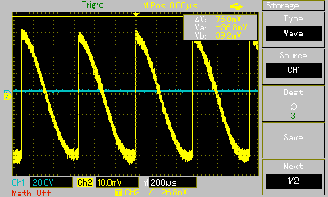
\includegraphics{Oszilloskop_0.pdf}
        \caption{Phasenverschiebung $\varphi = 0°$}
        \label{fig:0deg}
    \end{subfigure}
    \hfill
    \begin{subfigure}{0.48\textwidth}
        \centering
        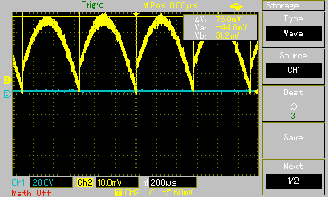
\includegraphics{Oszilloskop_90.pdf}
        \caption{Phasenverschiebung $\varphi = 90°$}
        \label{fig:90deg}
    \end{subfigure}
    \hfill
    \begin{subfigure}{0.48\textwidth}
        \centering
        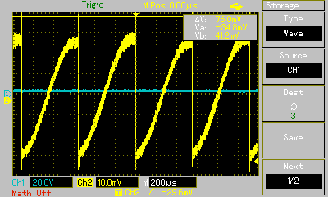
\includegraphics{Oszilloskop_180.pdf}
        \caption{Phasenverschiebung $\varphi = 180°$}
        \label{fig:180deg}
    \end{subfigure}
    \hfill
    \begin{subfigure}{0.48\textwidth}
        \centering
        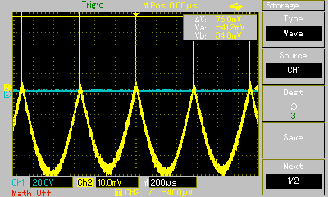
\includegraphics{Oszilloskop_270.pdf}
        \caption{Phasenverschiebung $\varphi = 270°$}
        \label{fig:270deg}
    \end{subfigure}
    \hfill
    \begin{subfigure}{0.48\textwidth}
        \centering
        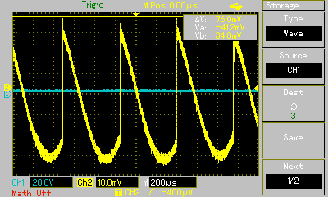
\includegraphics{Oszilloskop_315.pdf}
        \caption{Phasenverschiebung $\varphi = 315°$}
        \label{fig:315deg}
    \end{subfigure}    
\caption{Spannungsverläufe in Abhängigkeit der Phase zwischen Referenz und Signal.}
\end{figure}

\noindent
Die Abbildungen, zwischen denen jeweils $180°$ liegen sind an der x-Achse gespiegelt. Dies liegt an daran, dass die 
Referenzspannung immer genau das gleiche beziehungsweise immer genau das entgegengesetzte Vorzeichen wie die 
Signalspannung besitzt. So hat zum Beispiel die Referenzspannung in \autoref{fig:90deg} das gleiche Vorzeichen wie die 
Signalspannung, weshalb nur positive Komponenten existieren. So haben in \autoref{fig:180deg} haben Referenz- und 
Signalspannung genau entgegengesetzte Vorzeichen.
Gleiches lässt sich auch bei \autoref{fig:0deg} und \autoref{fig:180deg} beobachten.\\
\noindent
Im folgenden werden die Messdaten aud \autoref{tab:no_noise} und \autoref{tab:mit_noise} ausgewertet. Die gemessene 
Spannung wird gegen die eingestellte Phasenverschiebung aufgetragen. Über ein Pythonprogramm wird zu der 
theoretisch vorhergesagten Funktion \eqref{eqn:U_out} eine Kurve gefittet.

\begin{figure}[H]
    \includegraphics[width=\textwidth]{../build/no_noise.pdf}
    \caption{Nicht verrauschtes Signal.}
    \label{fig:fit_no_noise}
\end{figure}

\begin{figure}[H]
    \includegraphics[width=\textwidth]{../build/mit_noise.pdf}
    \caption{Verrauschtes Signal.}
    \label{fig:fit_mit_noise}
\end{figure}

\noindent
Zu sehen sind Wellen, die mithilfe der postulierten cosinus Welle beschrieben werden. yeet

\end{document}
